%!TEX program = xelatex

\documentclass[11pt,titlepage]{report}
%!TEX root = main.tex

\usepackage[T1]{fontenc}
\usepackage{lmodern}
\usepackage[svgnames]{xcolor}
\usepackage{fontspec} % XeLaTeX required!
\usepackage{graphicx}
\usepackage{circuitikz}
\usepackage{tikz}
\usepackage{pifont}
\usepackage[some]{background}
\usepackage{xltxtra} 
\usepackage{setspace}
\usepackage[absolute]{textpos}
\usepackage[latin1]{inputenc}
\usepackage[english]{babel}
\usepackage{graphicx}
\usepackage{wrapfig}
\usepackage{fullpage}
\usepackage[margin=1in]{geometry}
\usepackage{float}
\usepackage{url}
\usepackage{multicol}
\usepackage{hyperref}
\usepackage{titlepic}
\usepackage{standalone}
\usepackage{siunitx}
\usepackage{booktabs}
\usepackage{amsmath}
\usepackage{unicode-math}
\usepackage{verbatim}
\usepackage{enumitem}
\usepackage{listings}
\usepackage{multirow}
\usepackage{pgfplots}
\pgfplotsset{compat=1.8}
\usepackage{caption} 
\usepackage[parfill]{parskip}
\usepackage{import}
\usepackage[backend=bibtexu,texencoding=utf8,bibencoding=utf8,style=ieee,sortlocale=en_GB,language=auto]{biblatex}
\usepackage[strict,autostyle]{csquotes}
\usepackage[final]{pdfpages}
\usepackage{subcaption}
\usepackage{ifplatform}
%\captionsetup[table]{skip=10pt}


% Fix for includepdf bug in Mac OS X
\newcommand{\insertpdfpath}[1]{
	\ifwindows
	\newcommand{\insertpdf}[2]{\includepdf[pages=##1]{##2}}
	\else
	\newcommand{\insertpdf}[2]{\includepdf[pages=##1]{#1/##2}}
	\fi
}

%set fonts
\setmainfont[Ligatures=TeX]{Myriad Pro}
\setmathfont{Asana Math}
\setmonofont{Lucida Console}

\usepackage{titlesec, color}
\renewcommand{\familydefault}{\sfdefault} %set font family
\renewcommand{\arraystretch}{1.2} %set table vertical spacing
\setlength\parindent{0pt} %no paragraph indent
\hypersetup{ %setup hyperlinks
    colorlinks,
    citecolor=black,
    filecolor=black,
    linkcolor=black,
    urlcolor=black
}

%redesign chapter headings
\definecolor{gray75}{gray}{0.75}
\newcommand{\chapternumber}{\thechapter}
\newcommand{\hsp}{\hspace{20pt}}
\titleformat{\chapter}[hang]{\Huge\bfseries}{\chapternumber\hsp\textcolor{gray75}{|}\hsp}{0pt}{\Huge\bfseries}

%Redefine appendix headers
\renewcommand{\appendixname}{Appendix}
\renewcommand{\appendixtocname}{Appendices}
\renewcommand{\appendixpagename}{Appendices}

%For code listings
\definecolor{black}{rgb}{0,0,0}
\definecolor{browntags}{rgb}{0.65,0.1,0.1}
\definecolor{bluestrings}{rgb}{0,0,1}
\definecolor{graycomments}{rgb}{0.4,0.4,0.4}
\definecolor{redkeywords}{rgb}{1,0,0}
\definecolor{bluekeywords}{rgb}{0.13,0.13,0.8}
\definecolor{greencomments}{rgb}{0,0.5,0}
\definecolor{redstrings}{rgb}{0.9,0,0}
\definecolor{purpleidentifiers}{rgb}{0.01,0,0.01}


\lstdefinestyle{csharp}{
language=[Sharp]C,
showspaces=false,
showtabs=false,
breaklines=true,
showstringspaces=false,
breakatwhitespace=true,
escapeinside={(*@}{@*)},
columns=fullflexible,
commentstyle=\color{greencomments},
keywordstyle=\color{bluekeywords}\bfseries,
stringstyle=\color{redstrings},
identifierstyle=\color{purpleidentifiers},
basicstyle=\ttfamily\small}

\lstdefinestyle{c}{
language=C,
showspaces=false,
showtabs=false,
breaklines=true,
showstringspaces=false,
breakatwhitespace=true,
escapeinside={(*@}{@*)},
columns=fullflexible,
commentstyle=\color{greencomments},
keywordstyle=\color{bluekeywords}\bfseries,
stringstyle=\color{redstrings},
identifierstyle=\color{purpleidentifiers},
}

\lstdefinestyle{matlab}{
language=Matlab,
showspaces=false,
showtabs=false,
breaklines=true,
showstringspaces=false,
breakatwhitespace=true,
escapeinside={(*@}{@*)},
columns=fullflexible,
commentstyle=\color{greencomments},
keywordstyle=\color{bluekeywords}\bfseries,
stringstyle=\color{redstrings},
identifierstyle=\color{purpleidentifiers}
}

\lstdefinestyle{vhdl}{
language=VHDL,
showspaces=false,
showtabs=false,
breaklines=true,
showstringspaces=false,
breakatwhitespace=true,
escapeinside={(*@}{@*)},
columns=fullflexible,
commentstyle=\color{greencomments},
keywordstyle=\color{bluekeywords}\bfseries,
stringstyle=\color{redstrings},
identifierstyle=\color{purpleidentifiers}
}

\lstdefinestyle{xaml}{
language=XML,
showspaces=false,
showtabs=false,
breaklines=true,
showstringspaces=false,
breakatwhitespace=true,
escapeinside={(*@}{@*)},
columns=fullflexible,
commentstyle=\color{greencomments},
keywordstyle=\color{redkeywords},
stringstyle=\color{bluestrings},
tagstyle=\color{browntags},
morestring=[b]",
  morecomment=[s]{<?}{?>},
  morekeywords={xmlns,version,typex:AsyncRecords,x:Arguments,x:Boolean,x:Byte,x:Char,x:Class,x:ClassAttributes,x:ClassModifier,x:Code,x:ConnectionId,x:Decimal,x:Double,x:FactoryMethod,x:FieldModifier,x:Int16,x:Int32,x:Int64,x:Key,x:Members,x:Name,x:Object,x:Property,x:Shared,x:Single,x:String,x:Subclass,x:SynchronousMode,x:TimeSpan,x:TypeArguments,x:Uid,x:Uri,x:XData,Grid.Column,Grid.ColumnSpan,Click,ClipToBounds,Content,DropDownOpened,FontSize,Foreground,Header,Height,HorizontalAlignment,HorizontalContentAlignment,IsCancel,IsDefault,IsEnabled,IsSelected,Margin,MinHeight,MinWidth,Padding,SnapsToDevicePixels,Target,TextWrapping,Title,VerticalAlignment,VerticalContentAlignment,Width,WindowStartupLocation,Binding,Mode,OneWay,xmlns:x}
}

\lstdefinestyle{matlab}{
language=Matlab,
showspaces=false,
showtabs=false,
breaklines=true,
showstringspaces=false,
breakatwhitespace=true,
escapeinside={(*@}{@*)},
columns=fullflexible,
commentstyle=\color{greencomments},
keywordstyle=\color{bluekeywords}\bfseries,
stringstyle=\color{purpleidentifiers},
identifierstyle=\color{purpleidentifiers}
}

%defaults
\lstset{
basicstyle=\ttfamily\small,
extendedchars=false,
numbers=left,
numberstyle=\ttfamily\tiny,
stepnumber=1,
tabsize=4,
numbersep=5pt
}
\addbibresource{../../library/bibliography.bib}

\begin{document}

\chapter{Assignment 1}
\section{Labday 1}
\subsection{Report 1}
Let us consider the case where we want to calculate the channel impulse response when both the transmitter and receiver are placed into a closed room. The sound waves will theoretically infinitely reflect on the walls and cause an infinite impulse response (IIR). By making use of high school physics and MATLAB, we are able to approximate this channel impulse response. The room is defined by $\left\{(x,y) : 0 \le x \le 4, 0 \le y \le 4 \right\}$. The transmitter is located at $(1.2, 0.3)$ and the receiver at $(3.1, 3.3)$. If $r$ denotes the travelled distance, then the attenuation of the sound waves is given by
\[
	\alpha(r) = \beta / r^2.
\]
Figure~\ref{fig:ass-1-rep-1-refl} shows approximations of the impulse response and system response to a square wave for \num{24} and \num{2600} reflections for $\beta = 1$.

\begin{figure}[H]
	\centering
	\begin{subfigure}{0.49\textwidth}
		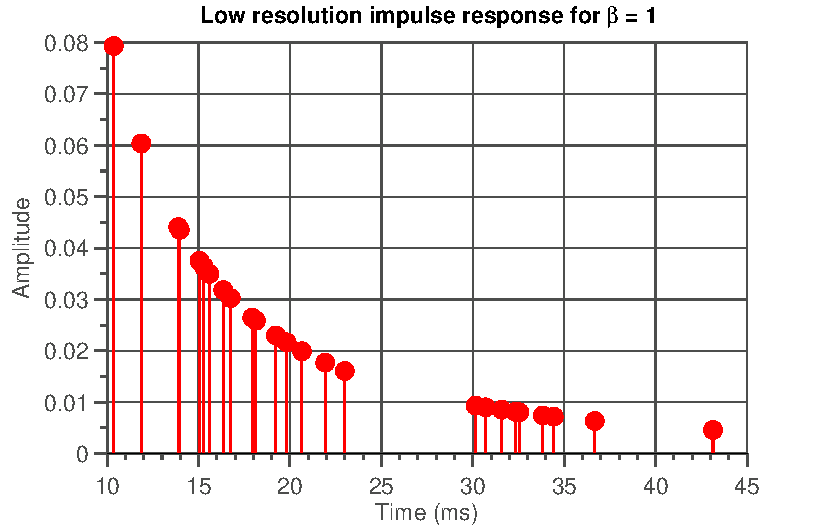
\includegraphics[width=\textwidth]{../../deliverable-7-resources/figures/ass-1/report-1/ass-1-report-1-impulse-response-2-copies-beta-1.pdf}
		\caption{\centering Low resolution impulse response approximation for $\beta=1$}
	\end{subfigure}
	\begin{subfigure}{0.49\textwidth}
		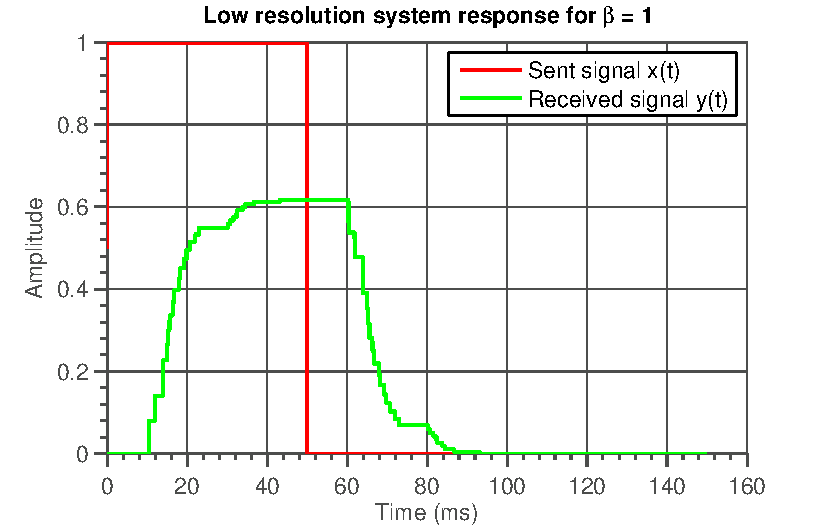
\includegraphics[width=\textwidth]{../../deliverable-7-resources/figures/ass-1/report-1/ass-1-report-1-system-response-2-copies-beta-1.pdf}
		\caption{\centering Low resolution system response approximation for $\beta=1$}
	\end{subfigure}
	\begin{subfigure}{0.49\textwidth}
		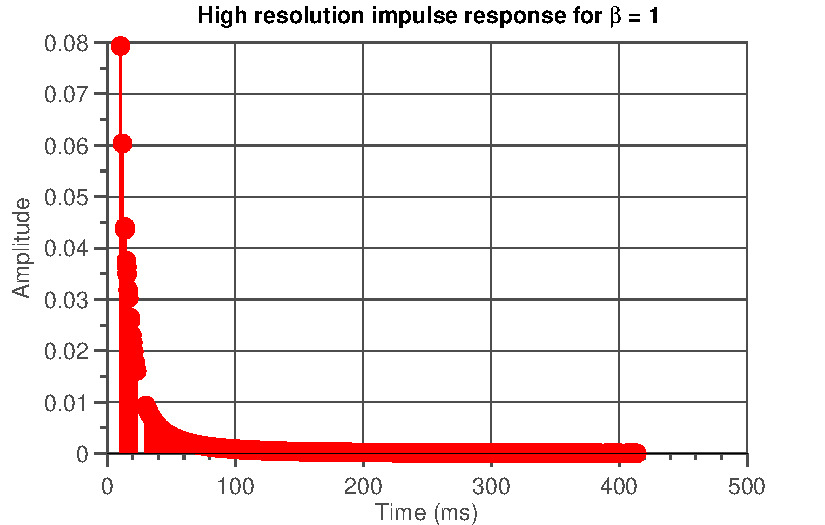
\includegraphics[width=\textwidth]{../../deliverable-7-resources/figures/ass-1/report-1/ass-1-report-1-impulse-response-25-copies-beta-1.pdf}
		\caption{\centering High resolution impulse response approximation for $\beta=1$}
	\end{subfigure}
	\begin{subfigure}{0.49\textwidth}
		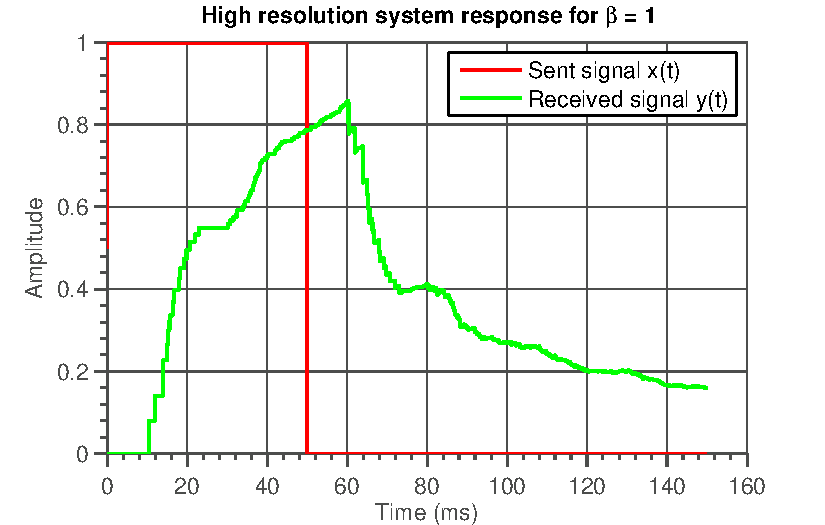
\includegraphics[width=\textwidth]{../../deliverable-7-resources/figures/ass-1/report-1/ass-1-report-1-system-response-25-copies-beta-1.pdf}
		\caption{\centering High resolution impulse response approximation for $\beta=1$}
	\end{subfigure}
	\caption{Low resolution (\num{24} reflections) and high resolution (\num{2600} reflections) impulse response and system response approximations}
	\label{fig:ass-1-rep-1-refl}
\end{figure}

\subsection{Report 2}
Here we consider a more general first-order IIR filter $\operatorname{\mathcal{Z}}\left\{h(t)\right\}=H(z) = (1+az^{-1})^{-1}$. Figure~\ref{fig:ass-1-rep-2-time} shows $h(t)$ for two different values of $a$. Figure~\ref{fig:ass-1-rep-2-z} shows $|H(\omega)|$ for two different values of $a$.

\begin{figure}[H]
	\centering
	\begin{subfigure}{0.49\textwidth}
		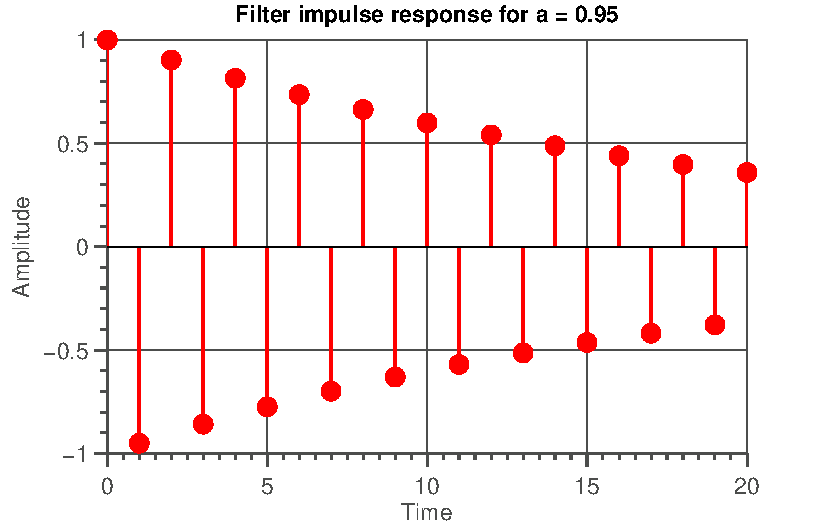
\includegraphics[width=\textwidth]{../../deliverable-7-resources/figures/ass-1/report-2/ass-1-report-2-a-positive.pdf}
	\end{subfigure}
	\begin{subfigure}{0.49\textwidth}
		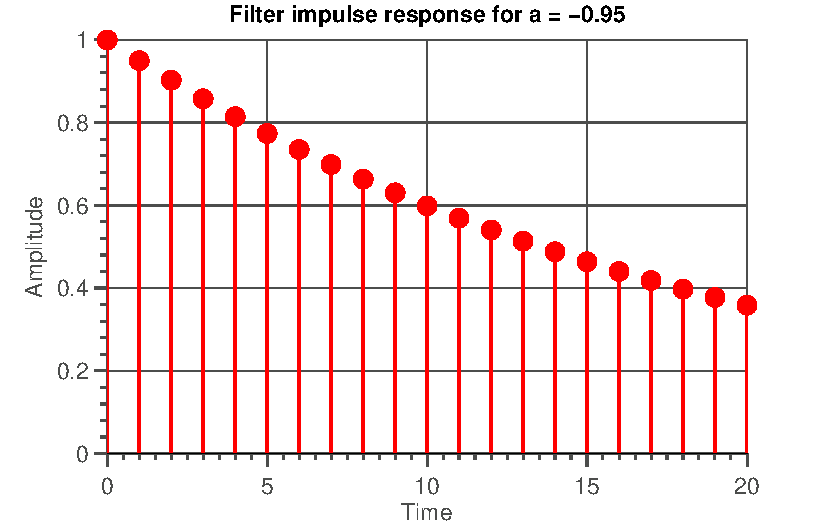
\includegraphics[width=\textwidth]{../../deliverable-7-resources/figures/ass-1/report-2/ass-1-report-2-a-negative.pdf}
	\end{subfigure}
	\caption{Impulse response of the first-order IIR filter for two values of $a$}
	\label{fig:ass-1-rep-2-time}
\end{figure}

\begin{figure}[H]
	\centering
	\begin{subfigure}{0.49\textwidth}
		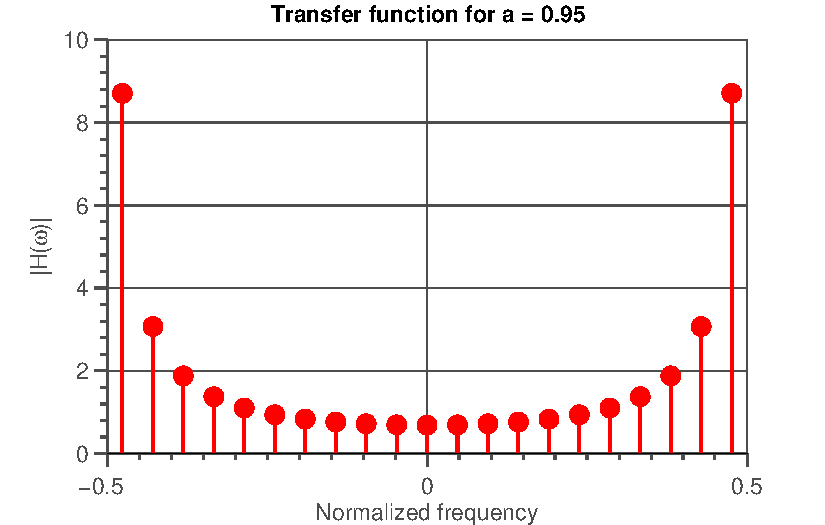
\includegraphics[width=\textwidth]{../../deliverable-7-resources/figures/ass-1/report-2/ass-1-report-2-a-positive-spectrum.pdf}
	\end{subfigure}
	\begin{subfigure}{0.49\textwidth}
		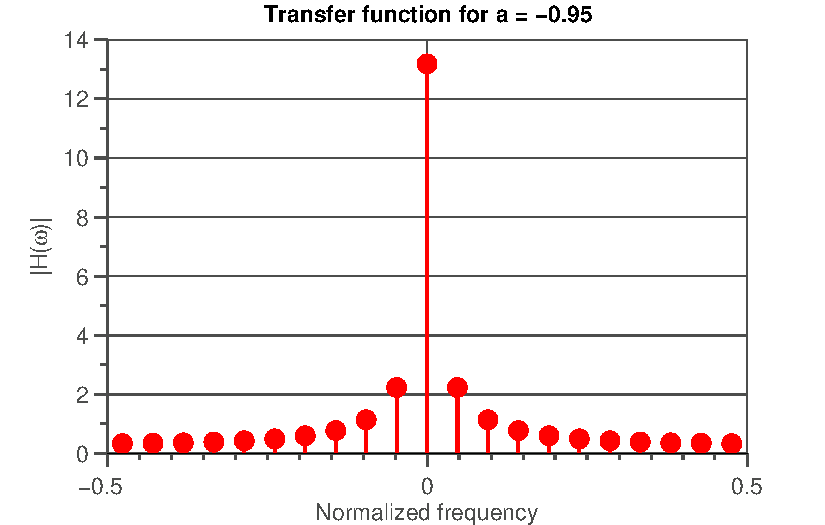
\includegraphics[width=\textwidth]{../../deliverable-7-resources/figures/ass-1/report-2/ass-1-report-2-a-negative-spectrum.pdf}
	\end{subfigure}
	\caption{Frequency response of the first-order IIR filter for two values of $a$}
	\label{fig:ass-1-rep-2-z}
\end{figure}

We see that for $a=0.95$ high frequencies are amplified. This corresponds to a form of a high-pass filter. For $a=-0.95$ low frequencies, particularly DC, are amplified and high frequencies are attenuated, which obviously corresponds to a low-pass filter.

In general, this filter is able to amplify or attenuate certain frequencies of an input signal. The value of $a$ determines exactly how an input signal is affected.

The reason that there is no MATLAB function FT or DTFT is the fact these functions require a evalution of an infinitely sized domain ($\mathbb{R}$ or $\mathbb{Z}$). A computer is obviously not able to do this, so approximations are required.

\subsection{Report 3}
Figure~\ref{fig:ass-1-rep-3} shows a time-domain representation of MATLAB's train signal (found by using the command \texttt{load train}).

\begin{figure}[H]
	\centering
	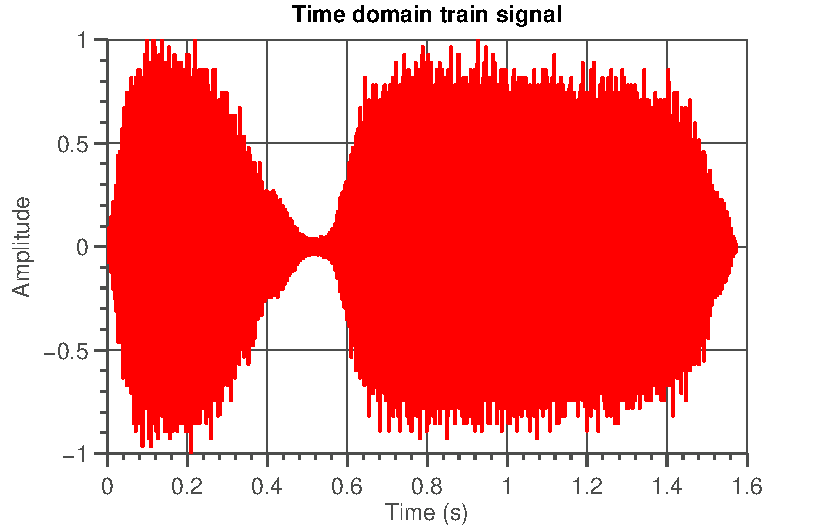
\includegraphics[width=0.6\textwidth]{../../deliverable-7-resources/figures/ass-1/report-3/ass-1-report-3.pdf}
	\caption{Time-domain representation of MATLAB's train signal}
	\label{fig:ass-1-rep-3}
\end{figure}

\subsection{Report 4}
Figure~\ref{fig:ass-1-rep-4} shows a time-frequency plot of MATLAB's train signals with intervals of \SI{20}{ms}. Note that the whistle-blows can easily be distinguished. The figure shows strong similarities with Figure~\ref{fig:ass-1-rep-3}. 

\begin{figure}[H]
	\centering
	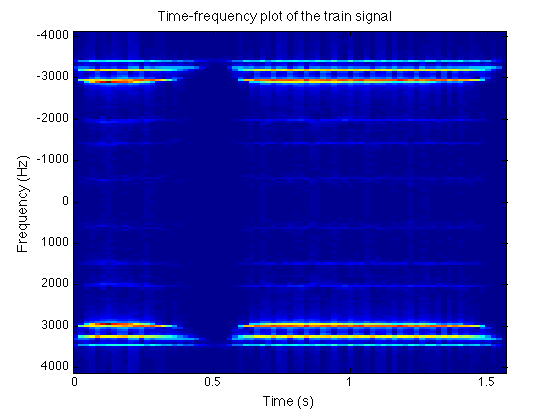
\includegraphics[width=0.6\textwidth]{../../deliverable-7-resources/figures/ass-1/report-4/ass-1-report-4.png}
	\caption{Time-frequency plot of MATLAB's train signal with intervals of \SI{20}{mc}}
	\label{fig:ass-1-rep-4}
\end{figure}

\subsection{Report 5 and 6}
\label{subsec:5-6}
The purpose of these reports is to show that zero padding interpolates a signal's spectrum. Let $h[n]$ be generated by the MATLAB command \texttt{[1  zeros(1,5)  0.9 zeros(1,5)  0.8]}. Figure~\ref{fig:ass-1-rep-5-6} shows the FFT of $h[n]$ for \num{13} samples, which is just $h[n]$, and for $5 \cdot 13$ samples, which is $h[n]$ extended by $4 \cdot 13$ zeros. One can easily see that the signal's spectrum is interpolated by addition of the zeros.

\begin{figure}[H]
	\centering
	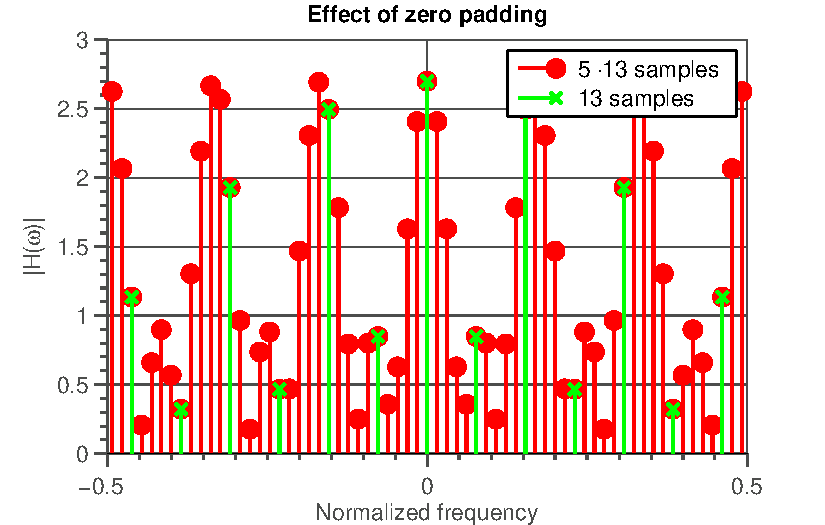
\includegraphics[width=0.6\textwidth]{../../deliverable-7-resources/figures/ass-1/report-5-6/ass-1-report-5-6.pdf}
	\caption{Frequency domain representation of the given impulse response with and without zero padding}
	\label{fig:ass-1-rep-5-6}
\end{figure}

\subsection{Report 7}
The purpose of this report is to show that
\[
	y[n] = x[n]*h[n] \Leftrightarrow Y(\omega) = X(\omega)H(\omega).
\]
We assigned MATLAB's train signal to $x[n]$ and the impulse response from Subsection \ref{subsec:5-6} to $h[n]$. Figure \ref{fig:ass-1-rep-7-conv} shows $|Y(\omega)|$ calculated by first convolving and then transforming and by first transforming and then multiplying. Inspection by eye shows that both methods result in the same spectrum. Therefore, we have verified the convolution property.

\begin{figure}[H]
	\centering
	\begin{subfigure}{0.49\textwidth}
		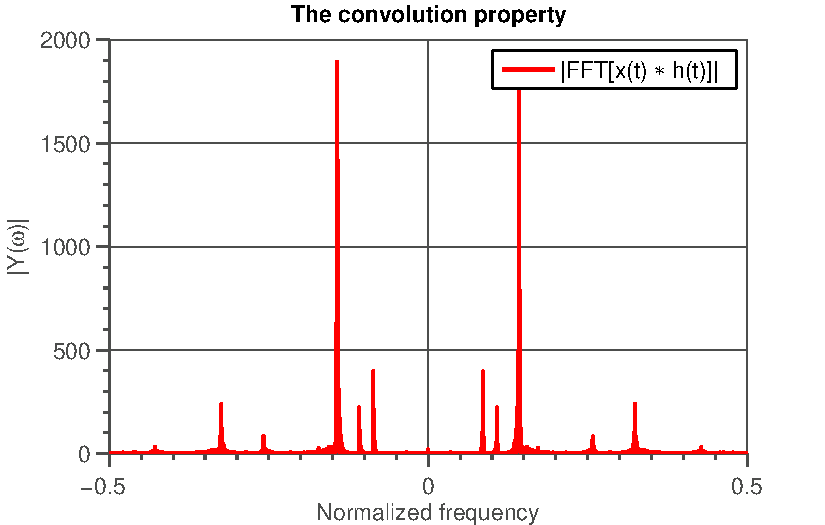
\includegraphics[width=\textwidth]{../../deliverable-7-resources/figures/ass-1/report-7/ass-1-report-7-convolution.pdf}
	\end{subfigure}
	\begin{subfigure}{0.49\textwidth}
		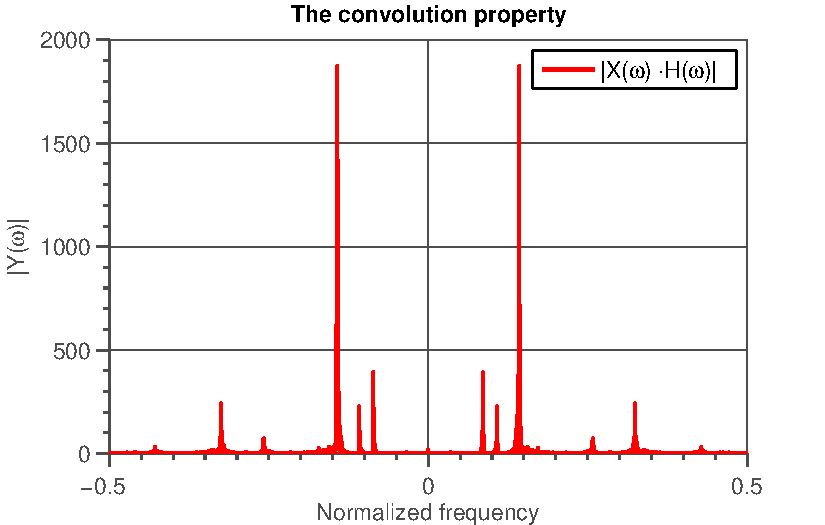
\includegraphics[width=\textwidth]{../../deliverable-7-resources/figures/ass-1/report-7/ass-1-report-7-multiplication.pdf}
	\end{subfigure}
	\caption{Comparison of spectra for testing the convolution property.}
	\label{fig:ass-1-rep-7-conv}
\end{figure}








\end{document}